% -------------------------------------------------------------------------------- %

\begin{exercise}

Quick-Hull ist ein auf einer ähnlichen Idee wie Quicksort basierender
Divide-And-Conquer-Algorithmus zum Auffinden einer endlichen Punktemenge im $\R^2$.
Er arbeitet wie folgt: Zunächst werden die beiden Punkte mit der größten und der
kleinsten $x$-Koordinate gesucht (sollte es mehrere Punkte mit kleinster/größter
$x$-Koordinate geben, so wähle denjenigen mit kleinster $y$-Koordinate).
Da diese Punkte Extremalpunkte sind, sind sie Bestandteil der konvexen Hülle. \\
Die beiden gefundenen Punkte bilden eine Gerade, die die Punktemenge in zwei
Teilmengen unterteilt: Die Punkte rechts von der Gerade und die Punkte links davon
(links und rechts ergeben sich aus dem Winkel zwischen dem Richtungsvektor der Geraden
und dem Vektor zwischen Anfangspunkt der Gerade und dem betrachtetem Punkt).
Diese beiden durch die Gerade getrennten Punktmengen werden nun von Quick-Hull
rekursiv betrachtet. Innerhalb der zu betrachtenden Punktmenge wird der Punkt $P$
gesucht, der die maximale Distanz zur Geraden hat. Dieser ist ebenfalls Teil der
konvexen Hülle. Das Dreieck bestehend aus den Endpunkten der Gerade und dem Punkt $P$
besteht aus drei Punkten, die alle zur konvexen Hülle gehören. Also können wir
alle Punkte im Inneren des Dreiecks bei weiteren Aufrufen des Algorithmus ignorieren. \\
Die Seiten des Dreiecks fungieren nun als neue Trenngeraden. Der Algorithmus
wird so lange wiederholt, bis nur noch die Endpunkte der Trenngerade Teil der
zu untersuchenden Punktemengen sind.

\begin{enumerate}[label = \alph*)]
  \item Illustrieren Sie die Arbeitsweise des Algorithmus anhand einer selbst
  gewählten Punktemenge mit mindestens 10 Punkten.
  \item Begründen Sie, warum $\Landau(n^2)$ die Worst-Case-Laufzeit von Quick-Hull ist.
\end{enumerate}

\end{exercise}

% -------------------------------------------------------------------------------- %


\begin{solution}

\phantom{}

\begin{enumerate}[label = \alph*)]
  \item Lies: Schritt 1 in grün, Schritt 2 in gelb, Schritt 3 in rot. \\

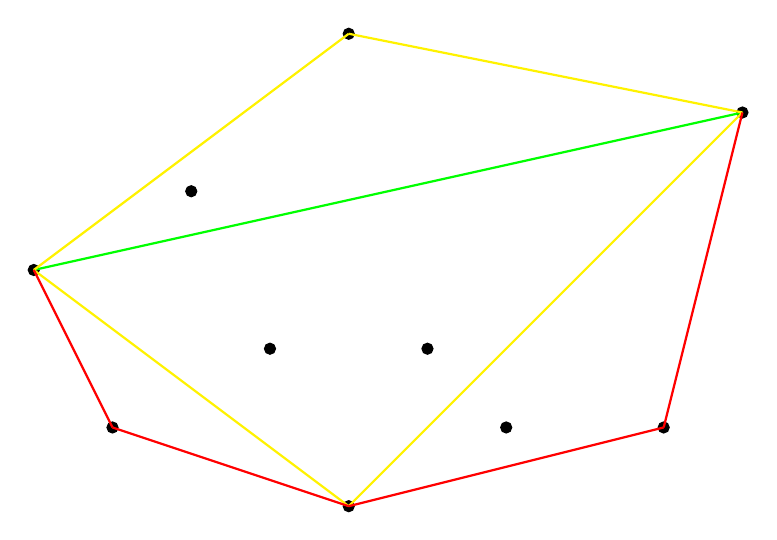
\begin{tikzpicture}
\filldraw[black] (0,0) circle (2pt);
\filldraw[black] (5,-1) circle (2pt);
\filldraw[black] (3,-1) circle (2pt);
\filldraw[black] (-2,-1) circle (2pt);
\filldraw[black] (-3,1) circle (2pt);
\filldraw[black] (6,3) circle (2pt);
\filldraw[black] (-1,2) circle (2pt);
\filldraw[black] (1,-2) circle (2pt);
\filldraw[black] (2,0) circle (2pt);
\filldraw[black] (1,4) circle (2pt);

\draw[green, thick] (-3,1) -- (6,3);

\draw[yellow, thick] (-3,1) -- (1,-2);
\draw[yellow, thick] (1,-2) -- (6,3);

\draw[yellow, thick] (-3,1) -- (1,4);
\draw[yellow, thick] (1,4) -- (6,3);

\draw[red, thick] (-3,1) -- (-2,-1);
\draw[red, thick] (-2,-1) -- (1,-2);

\draw[red, thick] (1,-2) -- (5,-1);
\draw[red, thick] (5,-1) -- (6,3);

\end{tikzpicture}

\item Mit jedem Dreieck, dass wir konstruieren, gewinnen wir zumindest einen
Punkt zu unser konvexen Hülle dazu. Also sind wir spätestens nach $n - 2$ Dreiecken fertig.
Für jedes Dreieck müssen wir schlimmsten Fall die maximale Distanz zur Dreieckskante
unter $n - 2$ Punkten bestimmen. Also kann unser Aufwand nicht schlimmer als $\Landau(n^2)$
werden.

\end{enumerate}

\end{solution}
